\section{Debugging}\label{debugging}

In any project which involves programming one is bound to do some debugging. This project is no exception. 
Debugging can be extremely frustrating because no one sees all the hours that go into finding the bugs, only the ones that do not (when the bug is not fixed). 
This appendix is an introductory guide to debugging finite difference (FD) solvers and RW implementations. It starts out with some general tips on how to handle error messages, and moves on to deal with FD and RW implementations. 
Finally, some words on how to debug the developed software are included.

\subsection{Compiler/syntax errors}
If you are programming in a compiled language like Fortran or C/C++ it is very easy to forget or misspell some syntax. 
Usually, the compiler will tell you what is wrong. 
Should it not do so, there are compiler options which provide extra information about syntactically correct but questionable looking code (-Wall). 
Some times one error results in several error messages. 
Start with the messages that are understandable, and recompile before checking out the other messages. \\

\noindent If you are building a larger project which requires linking, remember that packages must be linked in the correct order. 
For example; the Armadillo linear algebra library is backened by LAPACK and BLAS. 
In addition to linking the Armadillo library, both LAPACK and BLAS must be linked, and they must be linked in the correct order: 
\begin{lstlisting}
 g++ myprog.cpp -o myprog -O2 -larmadillo -llapack -lblas
\end{lstlisting}
Anything else will give very cryptic compiler errors. \\

Interpreted languages, like Python or MatLab, mostly include debuggers which provide extensive information about any errors in the code, read them thoroughly.

\subsection{Segmentation faults}
Segmentation fault is a very common abort message to get from C++. It means that the program has tried to access a part of the computer memory (RAM) which it is not allowed to access by the operating system. 
Interpreted languages will abort with a more informative error message, saying something about where the error was encountered. 
In a compiled language, ``Segmentation fault'' is all you get, which basically means that there is something wrong somewhere in your code. 
As an illustration, the terminal output below shows the output from a python- and C++- program for the same error:
\begin{lstlisting}
fredrik@Klokketiklokk:~/uio$ python segfault.py 
Traceback (most recent call last):
  File "segfault.py", line 3, in <module>
    b = sys.argv[1]
IndexError: list index out of range

fredrik@Klokketiklokk:~/uio$ ./segfault 
Segmentation fault (core dumped)
\end{lstlisting}

The gnu-compiler has an environment called gdb in which you can run your program. 
``gdb'' will catch segmentation faults and provide some information about where they were encountered. 
Furthermore, advanced editors like ``qt creator'' have built-in debuggers and the ability to place breakpoints in the code, making it possible to step through code line by line. \\
Some times though, the thing that works best is to print messages or key values at various places, signaling that a code block is finished. 
For example, making each function print its name when it is called will quickly identify problems. 

\subsection{Finite difference methods}
First and foremost: Do the discretization by hand. 
It will give valuable insight, which makes implementation and debugging a lot simpler. \\

\noindent There is one very important rule in programming in general: ``First make it work, then make right, then make it fast''. 
When solving PDEs numerically this principle is extra important. 
A numerical discretization scheme will (to my knowledge) either result in a main loop or a linear system which solves the equation. 
Regardless of the overall structure of the final program, this main block will be located somewhere, meaning that it should be implemented first. 
It can be made more efficient once it works. \\

\noindent Visualization is an invaluable tool while implementing a numerical PDE solver. 
Even though the code runs through all the steps without crashing, it does not have to be correct. 
This is illustrated in Figure \ref{appendix:visual_debugging}.
\begin{figure}[H]
 \centering
 \begin{subfigure}[t]{0.48\textwidth}
  \includegraphics[width=\textwidth]{Figures/incorrect_implementation.eps}
  \caption{Incorrect implementation}
 \end{subfigure}
 \begin{subfigure}[t]{0.48\textwidth}
  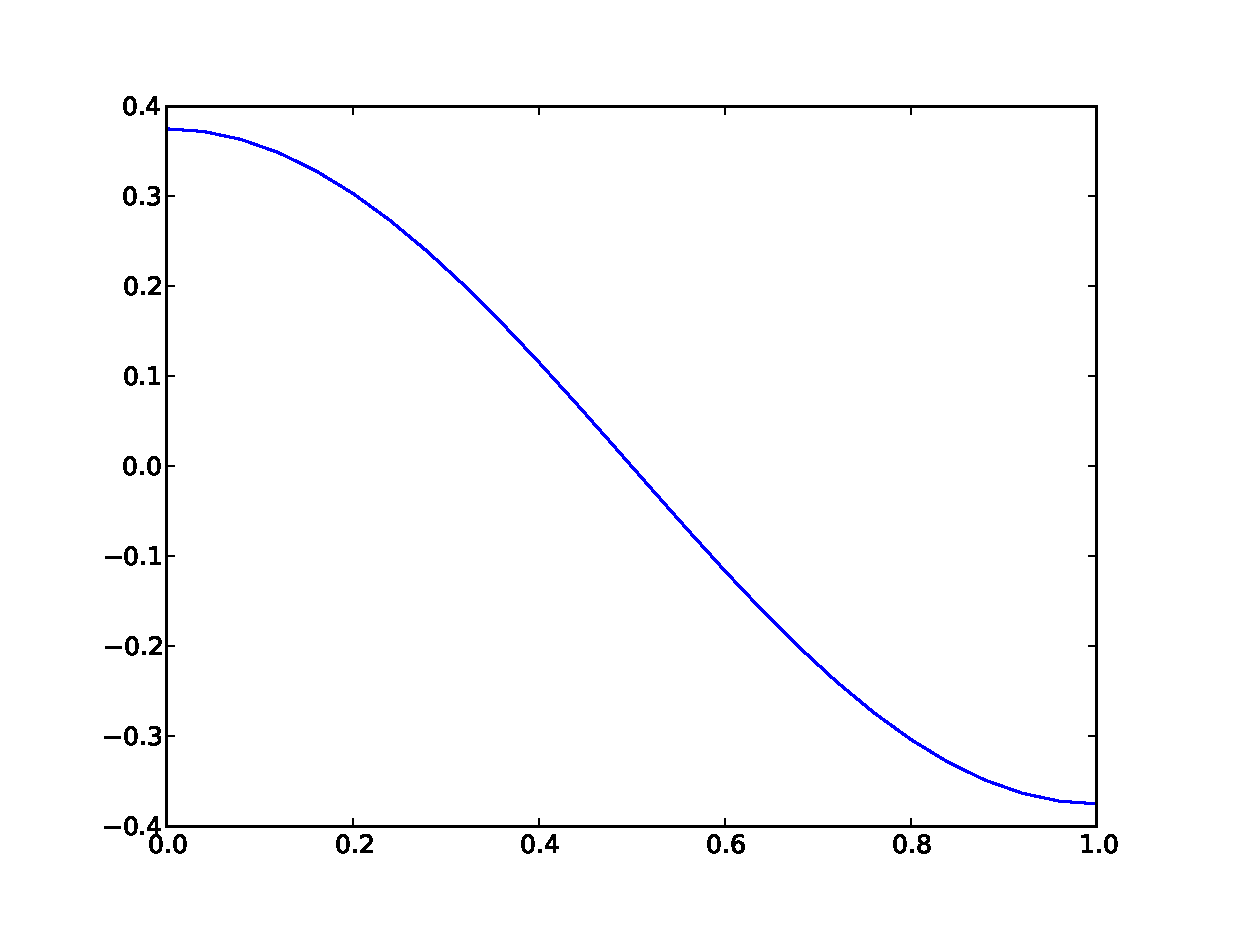
\includegraphics[width=\textwidth]{Figures/correct_implementation.eps}
  \caption{Correct implementation}
 \end{subfigure}
 \caption[Visual debugging]{Illustration of an implementation which does not crash the program, but is still clearly incorrect (a). (b) shows the correctly implemented version of the same time step.}
 \label{appendix:visual_debugging}
\end{figure}

 
\noindent At this point I would like to introduce rubber-duck debugging which is said to be invented by Dennis Ritchie, the developer of the C programming language. 
The story goes that he would keep a rubber duck at his desk and whenever he was stuck, would describe the code in detail (what each statement did and was supposed to do) to the rubber duck. 
Asking questions, and saying thing out loud forces you to think about things in a slightly different manner. \\

\noindent When the code seems to reproduce the intended results it is time to start the verification. 
This is where we make an error estimate and do some numerical analysis (the numerical stability of the scheme should, of course, be investigated prior to implementation). 
Making sure an implementation is correct is a lot harder than it sounds, but there are a few points that should be fulfilled:

\begin{itemize}
 \item Manufactured solution\\
 As was described earlier, the source term of the equation can be used to force almost any solution upon the equation. 
 
 \item Stationary solution\\
 This is a special type of manufactured solution. Using the source term, and initial condition, the solution can be forced to be constant. 
 If a scheme reproduces a stationary solution it conserves energy, which is very desirable.
 \item Exact numerical solution\\
 Depending on the discretization, it should be possible to find an exact solution to the discretized version of the PDE. 
 An example of this is found in chapter \ref{exact_numerical_solution}. 
 The scheme is expected to reproduce this solution to machine precision, but there are often several factors which limit the accuracy. 
 At the very least, the error should be significantly smaller than the largest error term. \\
 \item Convergence test\\
 These tests are often difficult to get right. 
 The principle is to verify that using a smaller discretization parameter results in a smaller error, and that the error is reduced by the expected amount. 
\end{itemize}

\noindent There are probably more ways to make sure that a finite difference scheme is working properly, but the ones listed will usually give a good implication.

\subsection{Random Walk and Monte Carlo methods}

While solving a PDE numerically, the intermediate calculations can be checked and verified. 
Since Monte Carlo methods are based on random numbers, the results of intermediate calculations will be random, making it impossible to verify them completely. 
Instead, some statistical properties of the random numbers can be verified. 
For example, using uniformly distributed random numbers will give a certain mean and standard deviation, while a Gaussian distribution will give another.
The random number generator should be tested in order to verify that these properties are reproduced to a reasonable accuracy. \\

\noindent Random walkers have some additional properties which can be tested. 
Both a one-dimensional and a two-dimensional random walk will fill all available space, given infinitely many time steps. 
Letting 4-5 walkers jump around for around $10^4$ time steps, and plotting their paths should give an indication of how well this property is reproduced. \\

\noindent Finally, it is very useful to specify a random seed. This will ensure that the random number generator produces the same sequence of numbers each simulation, which often makes testing easier. 
 
% As we have discussed earlier the fluctuations in a MC-model are usually of a magnitude $\frac{1}{\sqrt N}$ this is also smart to verify. \\
% Finally, you should absolutely have the possibility to set the random seed and check that two runs with the same random seed produces the exact same result and makes sure you are using a RNG with a large enough period. The xor-shift algorithm by Geroge Marsagla \cite{} has a period of around $10^{48}$ which usually is more than adequate.

\subsection{The developed software}

Since the developed software combines two solvers, it is of course very important to make sure that each solver is working properly. 
This can be verified by performing the tests mentioned earlier. 

While implementing the hybrid solver, there were four main points which either made the work easier, or would have made the work easier:

\begin{itemize}
 \item Unit testing\\
 This is a way to test a single unit of code, often a single function, and verify that it does exactly what it should do. \\
 \item Version control\\
 During implementation and testing, a lot of changes will be made to the code. It is surprisingly difficult to remember all the changes, which often means that functioning code will be lost. 
 Using version control software eliminates this problem. Version control software allows a developer to save snapshots of code with a comment, as well as some more advanced options. This allows for tracking of progress, committing working code before changes are made, and much more. Should some changes be made to a working piece of code, it can be reverted to the last working version.\\
 \item Make independent modules\\
 This applies to most code development. If the code is divided into independent modules, it is not only easier to test the code, it will also be much easier to reuse the code. \\
 As an example, the block tridiagonal solver has been implemented as a separate module, which since then has been used by Torbjørn Sæland in his masters thesis.\\
 \item Do not be nostalgic\\
 Because you are now using version control, there is no need to just comment out sections of code in case it is needed later. 
 This makes the rest of the code less messy, and reduces the risk of forgetting to remove something.
\end{itemize}

% 
% For some 2 months while working with this project I got really good results which seemed to verify all the important parts of the theory. 
% Unfortunately it turned out that, while individually both parts of the program did exactly what they were supposed to do (verified by various tests), the combination of the two parts was implemented wrong. 
% What actually happened was a finer and finer round-off rather than taking some number of steps with random walkers and combining the two models. 
% It turned out that I sent an empty array to the random walk class as a new initial condition for the current time-step. \\
% The moral behind this little story is that you should make 100\% sure that every part of every function you write does exactly what you think it does, and nothing else. 
% Furthermore, if you rewrite your code, you should remove the old parts as soon as possible. If you use some kind of version control software, which you definitely should, you will have older versions saved in the version control anyways. Do not be nostalgic and simply comment out the old parts just in case something, this makes your code very messy, and leaves the possibility of something slipping past you.
% 
% Another point to be made is that it will probably be helpful to construct the different parts of your code in such a way that they can be run as independently of each other as possible. 
% As an example, both the PDE-solver, its tridiagonal linear system solver and the spine object can with relatively small changes to the main-file be run independently. 
% This allows for easier testing of the various parts of the code, and makes it more likely that the code will be reused in other projects.

\subsection{Last resorts}

If nothing else seems to work, I like to try these techniques in order to get a fresh view on the problem.

First off all, doing some form of verification of intermediate steps by hand is often very useful. If everything seems to be implemented correctly, but the results are still wrong, it is time to really verify as much as possible. Try verifying indexing, counting, etc.

Changing parameters is often useful. As a rule of thumb, it is unwise to use ``simple'' parameter values, like zero or one, because values like these are often special cases which give simple effects. 
Changing a constant from one to a random value between zero and ten can often illustrate errors in parts of the code which has already been tested. 
Similarly, any matrix calculations done by hand should be done with matrices larger than $3\times 3$. 
It is much harder to recognize patterns in smaller matrices.

If neither of these work, try starting from scratch in a different programming language (preferably an interpreted language). The slight difference in syntax often reveals a lot of problems.

Finally, it often helps to get some distance from the problem. Work with something else for a couple of days, and come back with a fresh, and more critical view.

% While debugging (or any other repetitive task involving your own work) it is remarkably easy to become blind to your mistakes. 
% The psychology behind this is (probably) that you have a clear idea of what should happen in each statement, and so you read that in stead of what the statement actually says. 
% When it comes to proof-reading you can supposedly read backwards word by word, but can you do something similar when reading code? 
% While I have never tried reading my code backwards because a statement usually depends on the previous statement, I have tried doing hand-calculations for almost every statement. 
% Although hand calculations do not always show where things go wrong, they point out what variable or array entry etc. is wrong, and so the previous calculations can be checked. 
% For finite difference schemes one can reduce the number of spatial mesh points to something manageable like three or four, and then do the same calculations that you think the computer does. If the solution is a matrix you can pinpoint the invalid matrix-entries with this method.\\
% 
% Another very important point if you are stuck is to never use ``nice'' values. 
% If a parameter is set to zero or one just because it needs to be something, the probability that a potential problem disappears because it cancels out increases dramatically. 
% Similarly, never do matrix calculations for $3\times 3$ matrices. Use $4\times4$ matrices instead. The reasoning behind this is that banded matrices might fool you on $3\times 3$ matrices, making you think your problem is tridiagonal when it in fact is n-band diagonal for example.